\documentclass{book}
\usepackage{amsfonts}
\usepackage{amsmath}
\usepackage{graphicx}
\usepackage{epstopdf}
\usepackage{amssymb}
\usepackage{hyperref}
\usepackage{listings}
\usepackage{units}
\setcounter{chapter}{5}

\begin{document}
\chapter[Experimental Design III]{Experimental Design III: Standing Waves on Strings}

\section{Introduction}

Standing waves result from making waves that reflect back on themselves, or by
making waves on both ends of a string. When we were children we formed a type
of standing wave with jump ropes.
\begin{center}
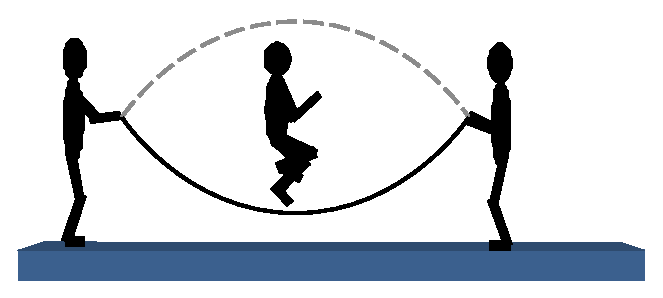
\includegraphics[natheight=3.749800in,natwidth=5.000400in,height=0.9262in,width=1.2306in]{Lab6_figs/JumpRope1stHar.eps}
\end{center}
This standing wave had a part that went up and down in the middle and two
parts that did not move much on each end (called nodes). But if you had a
bored kid, you might have seen a standing wave that looks like this.%
\begin{center}
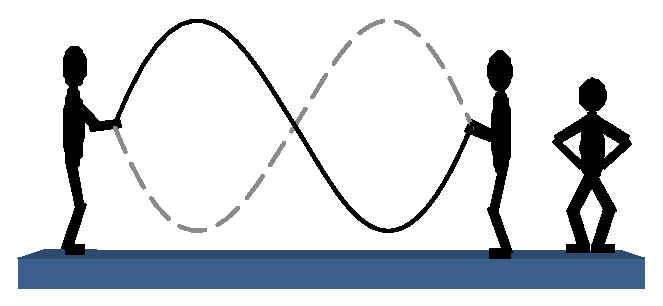
\includegraphics[natheight=3.749800in,natwidth=5.000400in,height=0.9446in,width=1.256in]{Lab6_figs/JumpRope2ndHar.eps}
\end{center}
This is not so good for jumping, but makes an interesting picture. The part in
the middle that does not seem to be moving is called a node. Really there are
also nodes on each end of the rope as well. So altogether there are three
nodes in this picture. We can make standing waves that have many nodes. If you
try this with a jump rope, you will find that the more nodes you have, the
faster you have to shake your end of the rope. Another way to say this is that
the frequency of your wave you are making must increase with the number of
nodes. This is part of today's model.

In the setup on your table, ring stands are holding strings, and there is an
oscillator on one end that has a frequency control box. The other end has a
pulley and a hanging mass to provide tension on the string.%
\begin{center}
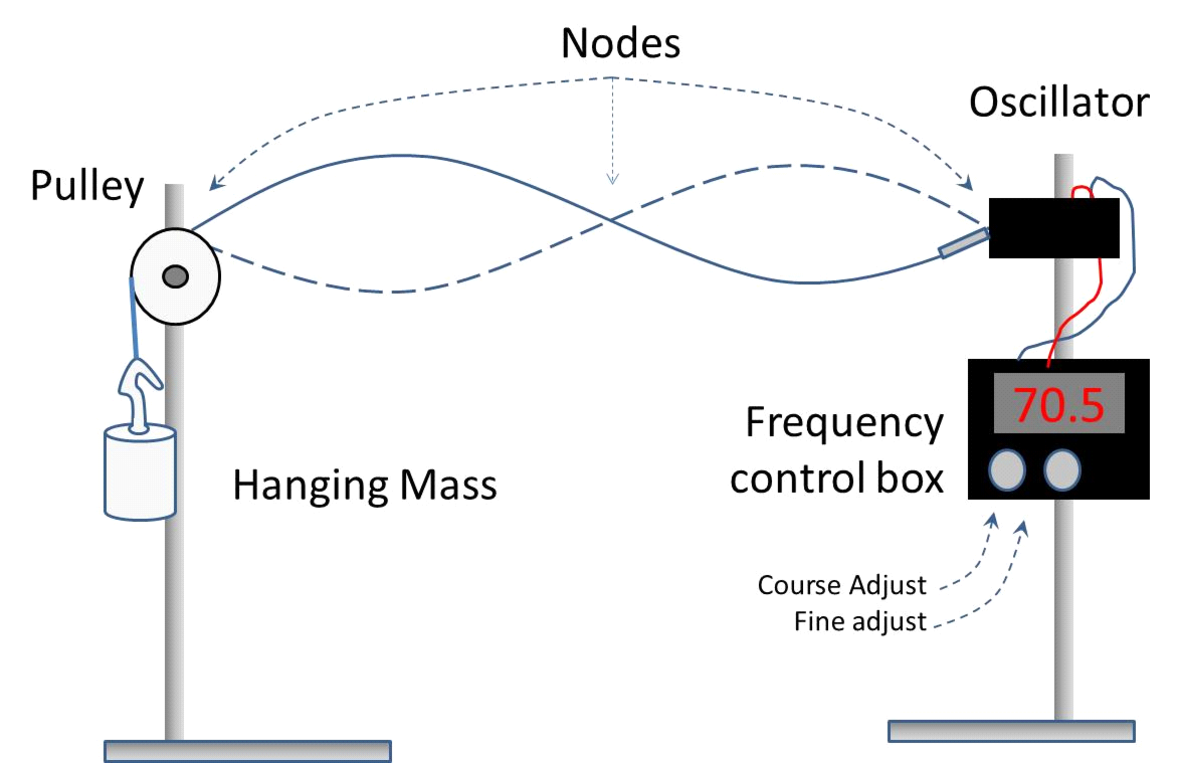
\includegraphics[natheight=1.907800in,natwidth=2.949000in,height=1.5451in,width=2.3753in]{Lab6_figs/StandingWaveonString.png}
\end{center}

Experimentally we find that not all frequencies will make standing waves. So
our model includes the idea that only some frequencies produce standing waves.
Our model also includes the idea that the weight of the string will change
which frequency will make a standing wave. If you play a stringed instrument,
you may have noticed that some strings are thicker than others. Thicker
strings have different standing wave frequencies than thinner strings. If you
study this model (some of you will in PH123), you can derive an equation that
tells which frequencies will work%
\begin{equation}
f=\frac{n}{2L}\sqrt{\frac{Mg}{\mu}}\label{tolinearize}
\end{equation}
where $n$ is an integer ($n=1,2,3\ldots$). This integer for strings is the
number of nodes minus one $n=n_{nodes}-1$. So you can form a standing wave,
then count the places that don't seem to move (remember the ends!) and
subtract one to find $n.$ The frequency that creates the standing wave should
be a function of $n.$ \textbf{Our model tells us that if we know }%
$n,$\textbf{\ we should be able to predict the frequency}. You will find that
for each way you can make a standing wave, a small range of frequencies will
make the standing wave, not just one, single frequency. But the frequency that
produces the largest standing wave is the one we want (biggest amplitude--or
the one for which the wave looks bigger) . That was the $f$ that was included
in forming our model equation. Of course there are other variables in our
equation, so we should find out what they are.

The quantity, $\mu,$ is the linear mass density. It is defined as mass of the
string divided by the length of the string. So $\mu$ tells us how massive the
string is.

The quantity, $L$ is the length of the string that is participating in the
waving, $g=9.8004\unit{m}/\unit{s}^2$ is the acceleration due to gravity, and $M$ is the hanging mass tied to
the end of the string beyond the pulley.

One way we could verify our model equation is to use it to predict one of the
input values. Let's use $\mu$. \textbf{The idea is to use our model equation
to somehow find }$\mu$\textbf{\ and then measure }$\mu$\textbf{\ to see if the
model equation prediction is good.}

It might be tempting to just solve the above equation for $\mu$ and report the
answer from one measurement. And of course that will work. But I want to see if you can use some of the things we learned.

We learned earlier that we can take more than one measurement, and use those
measurements together with a curve fit to solve for a fit parameter. I\ want
you to do this. The quantity $\mu$ should be in one of the fit parameters.
Then you can solve for $\mu$ using the fit parameter given by your Python
linear fit code. This is a more robust way to find $\mu,$ and it is the way I want you to proceed (Even
if you solve for $\mu$ several times and take a mean and standard
deviation--it will work and it is a good experimental technique--but I want to
see if you can find and use your linear least squares code, so using your code
gives the most points).

You may have to adjust the amplitude knob on the frequency controller for some
frequencies to keep the apparatus from shaking itself apart. The frequency
controller has a fine and a course frequency adjust knob, and a digital
frequency display.

\section{Assignment}

As a group design an experiment to test the model. Your design should
include the steps from lab 5.

\begin{enumerate}
\item Identify the system to be examined. Identify the inputs and
outputs. Describe your system in your lab notebook.

\item Identify the model to be tested. Express the model in terms of
an equation representing a prediction of the measurement you will make. Record
this in your lab notebook. (If you have not solved this problem in your PH121
class yet, call me over and we will go through it together).

\item Plan how you will know if you are successful in your experiment.
Plan graphs or other reporting devices. Record this in your lab notebook. For
today's lab, I will provide the frequency control box, oscillator, rope, and pulleys. If you need
other equipment, ask.

\item Rectify your equation if needed. Record this in your lab
notebook.

\item Choose ranges of the variables. Record this in your lab
notebook.

\item Plan the experimental procedure. Record this in your lab
notebook.

\item Perform the experiment. Record this in your lab notebook. Go
through all the steps of performing an experiment. End with a conclusion that
clearly states whether your experiment supported the model, falsified the
model, or, if neither was possible, try to explain why.
\end{enumerate}



\end{document}
